\documentclass[12pt]{article}
\usepackage{graphicx}
\begin{document}
\title{Pipeline RISC-V Processor}
\author{Yanjie Xu 71002946}
\maketitle
\section{Introduction}
\subsection{block diagram}
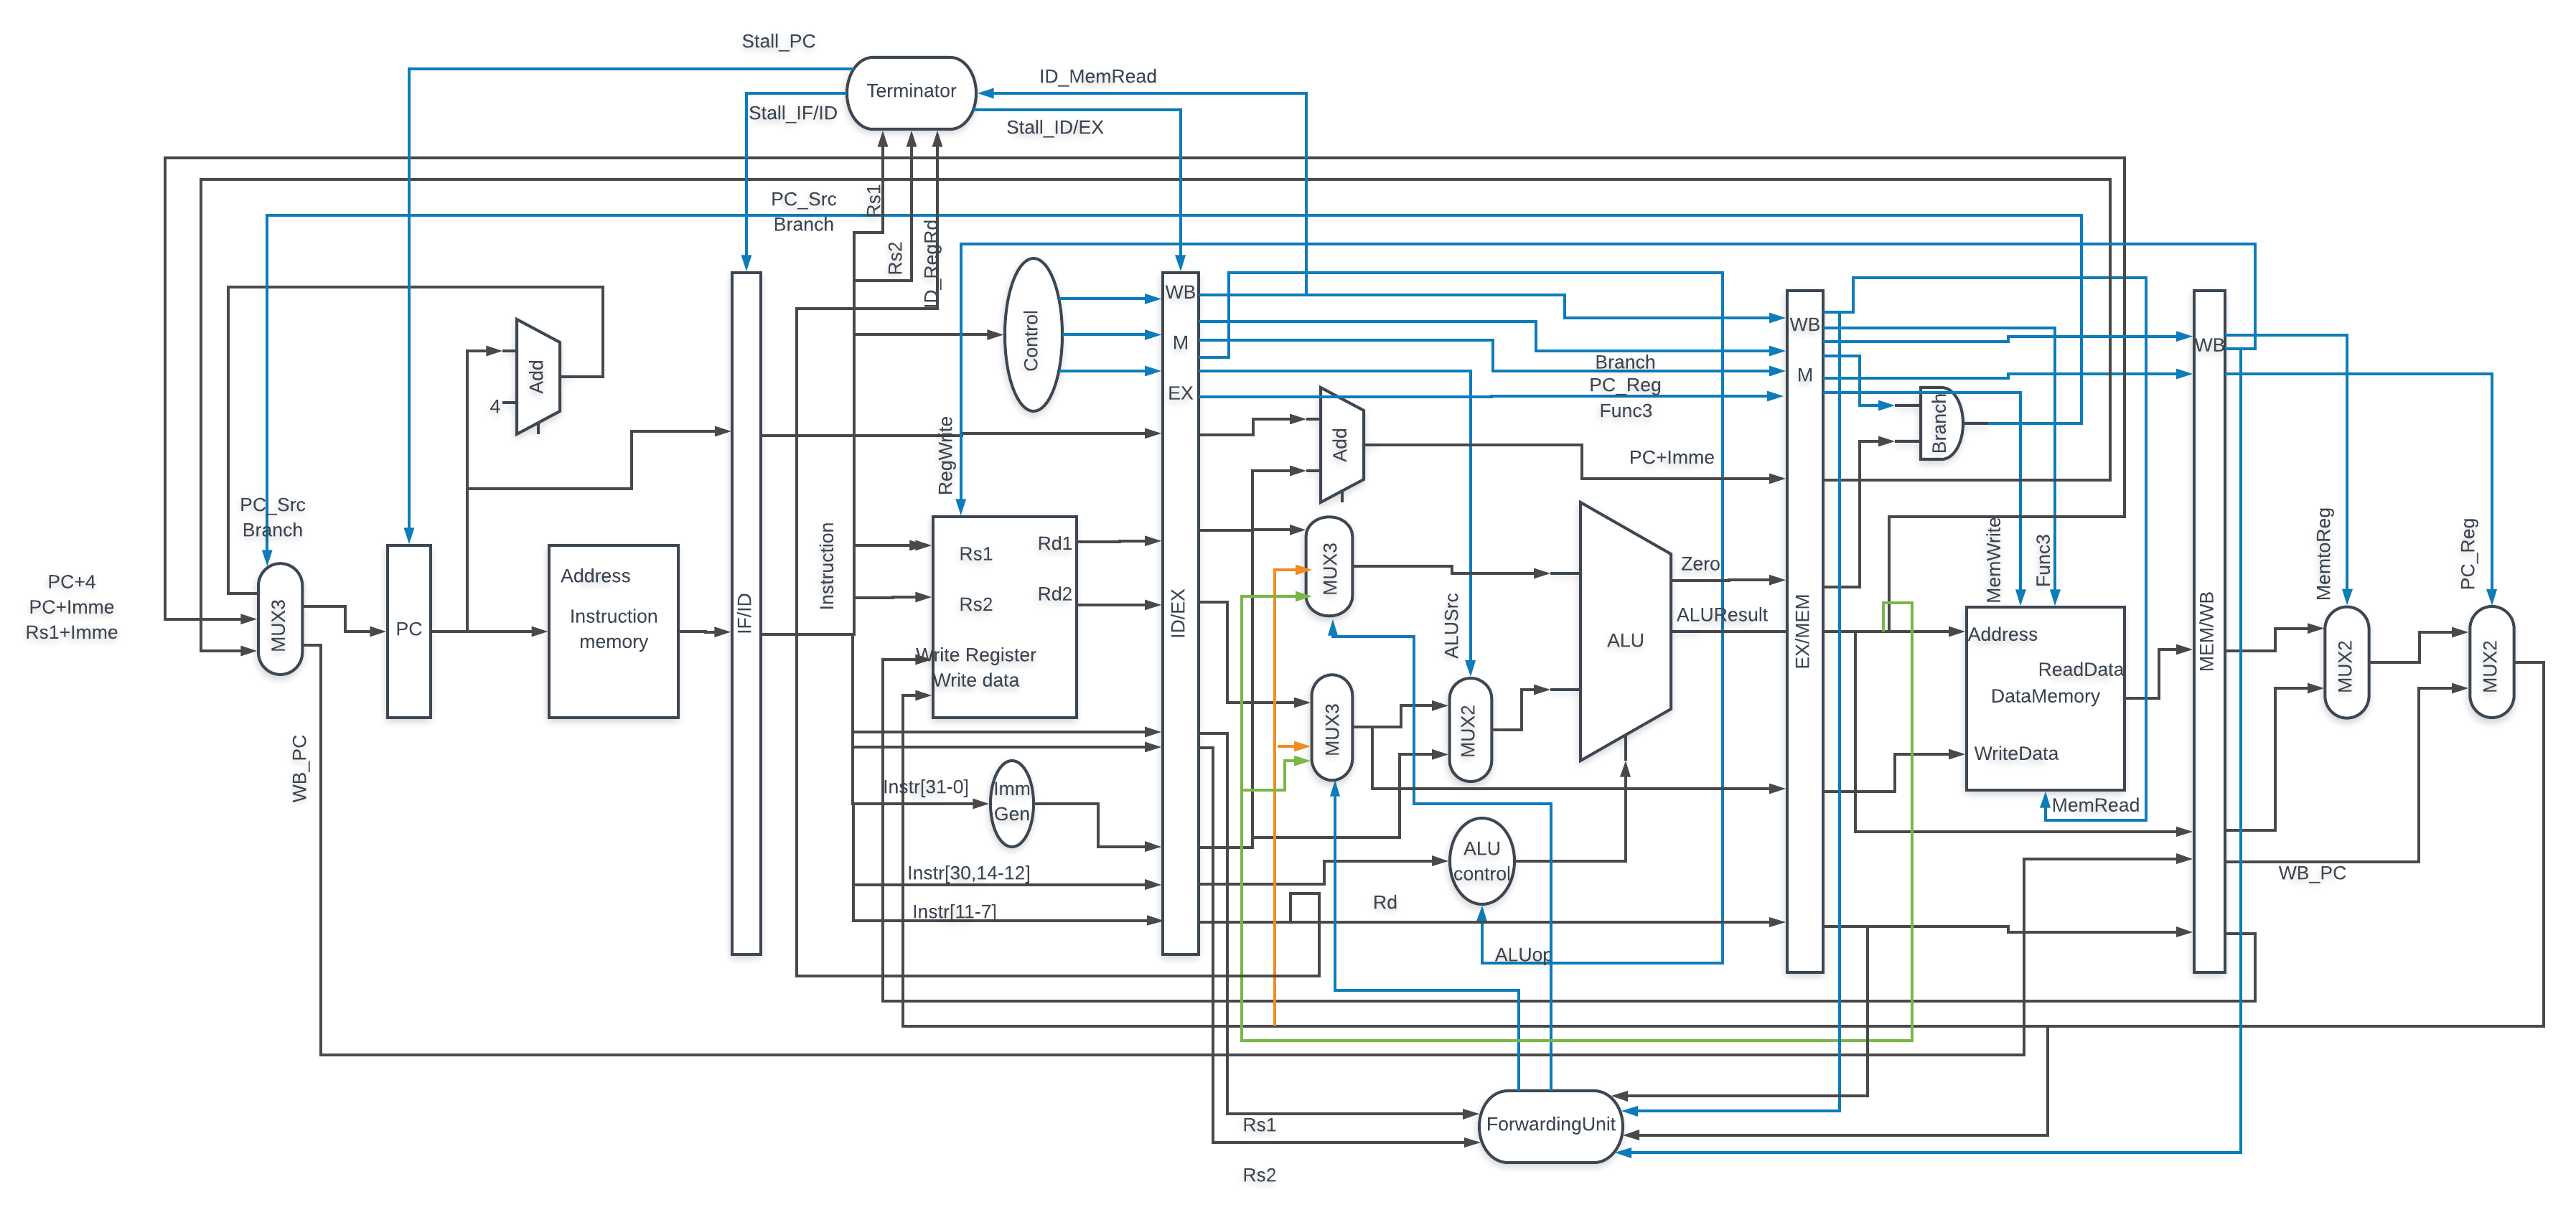
\includegraphics[width=\linewidth]{dia1.png}

\subsection{Block Brief Explaination}
The pipeline datapath used the same modules which used in the single cycle processor datapath. In addtion, the pipeline design added multiple registers which help store instructions information, forwarding unit and hazard detection unit\\\\
\textbf{IF/ID, ID/EX, EX/MEM, MEM/WB Registers}\\
In this pipeline processor design, these four registers function as storing current instruction and pass into the next register. In this way, one instruction can be finished in one cycle, there fore increased throughput.\\\\
\textbf{Forwarding Unit and Hazard Detection Unit}\\
Since this processor is a pipeline processor, it cannot avoid structural hazard or data hazard if there are multiple instruction process at the same time. However, by forwarding data from EM/MEM stage, and MEM/WB stage, the data hazard can be avoided. In addition, the hazard detection unit will stall the processor if there is a structural hazard, for example: load and store operation.\\




\section{Simulated Waveform}
The following waveform is the simulation result from 0 ns to 1000ns\\
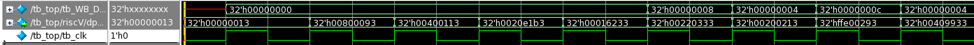
\includegraphics[width=\linewidth]{1.png}
\centerline{result, instruction,clock}\\
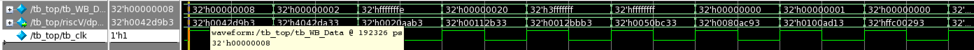
\includegraphics[width=\linewidth]{2.png}
\centerline{result, instruction,clock}\\
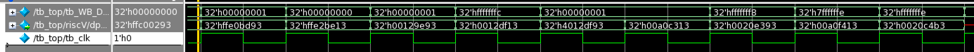
\includegraphics[width=\linewidth]{3.png}
result, instruction,clock\\
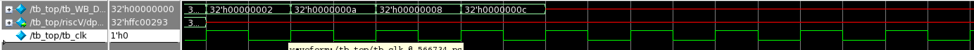
\includegraphics[width=\linewidth]{4.png}
result, instruction,clock\\
\section{Pipeline Synthesis Report}
\subsection{Critical Path}
  Timing Path Group 'clk'\\
  -----------------------------------\\
  Levels of Logic:              43.00\\
  Critical Path Length:          2.90\\
  Critical Path Slack:           1.09\\
  Critical Path Clk Period:      4.00\\
  Total Negative Slack:          0.00\\
  No. of Violating Paths:        0.00\\
  Worst Hold Violation:          0.00\\
  Total Hold Violation:          0.00\\
  No. of Hold Violations:        0.00\\
  -----------------------------------\\
  \subsection{Area}
 Area
  -----------------------------------\\
  Combinational Area:     9181.460322\\
  Noncombinational Area:  8054.586054\\
  Buf/Inv Area:            653.658370\\
  Total Buffer Area:           292.27\\
  Total Inverter Area:         361.39\\
  Macro/Black Box Area:      0.000000\\
  Net Area:               6129.390179\\
  -----------------------------------\\
  Cell Area:             17236.046377\\
  Design Area:           23365.436556\\

\section{Single Cycle Synthesis Report}
\subsection{Critical Path}
Timing Path Group 'clk'\\
  -----------------------------------\\
  Levels of Logic:              19.00 \\
  Critical Path Length:          5.70\\
  Critical Path Slack:          -3.72\\
  Critical Path Clk Period:      4.00\\
  Total Negative Slack:     -59235.94\\
  No. of Violating Paths:    17417.00\\
  Worst Hold Violation:          0.00\\
  Total Hold Violation:          0.00\\
  No. of Hold Violations:        0.00\\
  -----------------------------------\\
  \subsection{Area}
  Area\\
  -----------------------------------\\
  Combinational Area:    92205.985047\\
  Noncombinational Area:\\
                        115263.711104\\
  Buf/Inv Area:           5812.273369\\
  Total Buffer Area:          2657.84\\
  Total Inverter Area:        3154.44\\
  Macro/Black Box Area:      0.000000\\
  Net Area:             160072.172072\\
  -----------------------------------\\
  Cell Area:            207469.696151\\
  Design Area:          367541.868223\\
\section{Pipeline and Single cycle processor Comparison an d Discussion }
From the above chart we can see that: \\
1. The pipeline design eliminated most of the negative critical path slack and push the critical path slack to 1.09. \\\\
2. The pipeline design shortens the critical path length from 5.70 to 2.90 cycle.\\\\
3. The area used in pipeline design is significently smaller than the area in the single. The design area in single cycle is 367541.868223 and the cell area is 207469.696151.  23365.436556The design area in pipeline design is 17236.046377 and the cell area is  23365.436556\\

In conclusion, the pipeline design reduced the slack, increased the clock speed, shorted the critical path length, and reduced the design area. 23365.436556
\end{document}
